\documentclass[12pt,a4paper]{ctexart}

% --- 1. 页面与排版设置 ---
\usepackage{geometry}
\geometry{left=3.18cm, right=3.18cm, top=2.54cm, bottom=2.54cm}
\usepackage{setspace}
\onehalfspacing
\usepackage{enumitem}
\usepackage{graphicx}

% --- 2. 字体设置 (核心修改) ---
\usepackage{fontspec}

% 2.1 全局英文字体设置:Times New Roman
% 这将影响正文、标题、题注中的所有英文
% AutoFakeBold=true 是为了防止某些系统找不到粗体文件,通常 Windows 下不需要,但加上更保险
\setmainfont{Times New Roman}[AutoFakeBold=true]

% 2.2 代码块字体:模仿 MATLAB R2025
% 英文:Consolas
\setmonofont{Consolas}[Scale=0.95]
% 中文:微软雅黑
\setCJKmonofont{Microsoft YaHei}

% --- 3. 题注设置 (新增) ---
\usepackage{caption}
% font={small} : 题注字号通常比正文小一号
% labelfont={bf} : 标签 (如 "Listing 1") 加粗
% textfont={rm}  : 强制内容使用衬线字体 (即 Times New Roman),防止被 theme 篡改为无衬线
\captionsetup{
    font={small, rm}, 
    labelfont={bf},
    labelsep=quad
}

% --- 4. 页眉页脚设置 ---
\usepackage{fancyhdr}
\pagestyle{fancy}
\fancyhf{}                      
\cfoot{\thepage}                
\renewcommand{\headrulewidth}{0pt} 

% --- 5. 数学公式与颜色 ---
\usepackage{amsmath}
\usepackage{amssymb}
\usepackage{xcolor}

% --- 6. 代码块设置 (MATLAB 风格) ---
\usepackage{listings}

\definecolor{mKeyword}{RGB}{0, 0, 255}       
\definecolor{mString}{RGB}{160, 32, 240}     
\definecolor{mComment}{RGB}{34, 139, 34}     
\definecolor{mBackground}{RGB}{255, 255, 255} 

\lstset{
    language=Matlab,
    % 【修改点】将 \small 改为 \zihao{5},即五号字
    basicstyle=\zihao{5}\ttfamily,    
    keywordstyle=\color{mKeyword},
    commentstyle=\color{mComment},
    stringstyle=\color{mString},
    numbers=left,
    % 行号可以稍微再小一点,比如 \zihao{-5} (小五号) 或 \tiny
    numberstyle=\tiny\color{gray}\fontspec{Consolas},
    frame=single,
    breaklines=true,
    showstringspaces=false,
    backgroundcolor=\color{mBackground}
}

% --- 7. 标题格式定制 ---
\ctexset{
    section = {
        % \bfseries 会让中文用黑体,英文用 Times New Roman Bold
        format = \large\bfseries, 
        number = \arabic{section},
        name = {,},
        aftername = \quad
    },
    subsection = {
        format = \normalsize\bfseries,
        number = \arabic{section}.\arabic{subsection},
        name = {,},
        aftername = \quad
    }
}

\setlength{\parindent}{2em}

\begin{document}

% --- 封面 ---
\begin{center}
    \thispagestyle{empty}
    % \vspace*{1cm}
    {\Large \textbf{实验报告}} \\
    \vspace{0.5cm}
    代卓远 \\
    \vspace{0.5cm}
    2025210205,机械工程系,机研52 \\
    \vspace{0.5cm}
    (2026年1月4日)
    \vspace{0.5cm}
\end{center}


% --- 正文 ---

\section{题目}
实验目的:病态线性代数方程组的求解

问题:设$H_n=[h_ij]\in R^{n\times n}$是$n$阶Hilbert矩阵,即$$h_{ij}=\frac1{i+j-1},$$$x=(1,1,\cdots,1)^T\in R^n,\:b_n=H_nx.$。

(1)对$n=2,3,4,\cdots$,计算条件数$\mathrm{cond}(H_n)_1$,分析$\mathrm{cond}(H_n)_1$作为$n$的函数如何变化(用图表示);

(2)对$n=6$,用LU分解方法、Jacobi迭代法、SOR迭代法(取$\omega=1,1.25,1.5$等)以及共轭梯度法求解$H_nx=b_n$,计算几种方法的误差,选用适当的范数,列表表示结果, 结论如何;

(3)逐步增大$n$,用(2)中的方法求解,观察误差的变化($n$多大时绝对误差达到$100\%$,即连一位有效数字都没有了)(选用适当的范数,用图和表表示)。

\section{算法设计}

    \subsection{条件数计算(第一问)}
    对于$n$阶Hilbert矩阵$H_n = [h_{ij}] \in R^{n \times n}$(其中 $h_{ij} = \frac{1}{i+j-1}$),其1-范数条件数定义为:
    \begin{equation}
        \mathrm{cond}(H_n)_1 = \|H_n\|_1 \cdot \|H_n^{-1}\|_1
    \end{equation}

    其中,矩阵的1-范数(列范数)计算公式为:
    \begin{equation}
        \|A\|_1 = \max_{j} \sum_{i} |a_{ij}|
    \end{equation}

    由于$H_n$是对称矩阵,其1-范数与$\infty$-范数(行范数)数值相等。计算$n=2,3,\dots$时的条件数并作图分析。

    \subsection{方程组求解算法(第二问)}
    针对方程组 $H_n x = b_n$,采用以下方法求解:

    \subsubsection{LU分解法}
    若$A$的各阶顺序主子式均非零,存在唯一的单位下三角矩阵$L$和上三角矩阵$U$使得$A=LU$。
    分解公式如下 :
    \begin{align}
        u_{ij} &= a_{ij} - \sum_{k=1}^{i-1} l_{ik}u_{kj}, \quad (j = i, \dots, n) \\
        l_{ji} &= \frac{1}{u_{ii}} \left( a_{ji} - \sum_{k=1}^{i-1} l_{jk}u_{ki} \right), \quad (j = i+1, \dots, n)
    \end{align}
    求解$Ax=b$转化为求解$Ly=b$和$Ux=y$。

    \subsubsection{Jacobi迭代法}
        迭代公式为:
            \begin{equation}
                x^{(k+1)} = D^{-1}(b + Lx^{(k)} + Ux^{(k)})
            \end{equation}
    
    \subsubsection{SOR迭代法}
        选取松弛因子$\omega$,迭代公式为:
        \begin{equation}
            x^{(k+1)} = (1-\omega)x^{(k)} + \omega D^{-1}(b + Lx^{(k+1)} + Ux^{(k)})
        \end{equation}

        收敛的必要条件是$\omega \in (0, 2)$。
    
    \subsubsection{共轭梯度法}
        适用于对称正定矩阵。取初值$x^{(0)}$,令 $p^{(0)} = r^{(0)} = b - Ax^{(0)}$。

        第$k$步迭代步骤如下 :
        \begin{equation}
        \begin{aligned}
            \alpha_k &= \frac{(r^{(k)}, r^{(k)})}{(Ap^{(k)}, p^{(k)})} \\
            x^{(k+1)} &= x^{(k)} + \alpha_k p^{(k)} \\
            r^{(k+1)} &= r^{(k)} - \alpha_k Ap^{(k)} \\
            \beta_k &= \frac{(r^{(k+1)}, r^{(k+1)})}{(r^{(k)}, r^{(k)})} \\
            p^{(k+1)} &= r^{(k+1)} + \beta_k p^{(k)}
        \end{aligned}
        \end{equation}

    \subsection{误差分析(第三问)}
    定义数值解 $\tilde{x}$ 的相对误差为 $\frac{\|\tilde{x} - x^*\|}{\|x^*\|}$。
    根据误差分析定理,当系数矩阵存在扰动时,误差界与条件数$\mathrm{cond}(A)$成正比。对于Hilbert矩阵,由于$\mathrm{cond}(H_n)$极大,预计当$n$增大到一定程度(如$n \ge 12$),计算结果将完全失效。

\section{求解}

    \subsection{程序(注释)}

    \begin{lstlisting}
    function experiment()
        % 病态Hilbert矩阵实验
        clc; clear; close all;

        %% 1. 条件数分析
        fprintf('1. 条件数分析\n');
        n_cond_range = 2:16;
        conds = zeros(size(n_cond_range));
        
        for i = 1:length(n_cond_range)
            n = n_cond_range(i);
            H = hilb(n);
            % 1-范数条件数
            conds(i) = cond(H, 1); 
        end
        
        % 绘制条件数变化图
        figure(1);
        semilogy(n_cond_range, conds, '-bo', 'LineWidth', 1.5);
        title('Hilbert矩阵条件数cond(H)_1随n的变化');
        xlabel('矩阵阶数n');
        ylabel('条件数(对数坐标)');
        grid on;

        %% 2. n=6时的求解与误差计算
        fprintf('2. n=6时的求解误差\n');
        n = 6;
        [H, b, x_true] = setup_problem(n);
        
        % (1) LU分解法
        x_lu = solve_lu_manual(H, b);
        err_lu = norm(x_lu - x_true, inf) / norm(x_true, inf);
        
        % (2) Jacobi迭代法
        [x_jac, iter_jac] = solve_jacobi(H, b);
        err_jac = norm(x_jac - x_true, inf) / norm(x_true, inf);
        
        % (3) SOR迭代法
        omegas = [1.0, 1.25, 1.5];
        err_sor = zeros(length(omegas), 1);
        iters_sor = zeros(length(omegas), 1);
        for i = 1:length(omegas)
            [x_s, k_s] = solve_sor(H, b, omegas(i));
            err_sor(i) = norm(x_s - x_true, inf) / norm(x_true, inf);
            iters_sor(i) = k_s;
        end
        
        % (4) 共轭梯度法
        [x_cg, iter_cg] = solve_cg(H, b);
        err_cg = norm(x_cg - x_true, inf) / norm(x_true, inf);
        
        % 输出结果表格
        fprintf('%-15s %-10s %-15s\n', '方法', '迭代次数', '相对误差');
        fprintf('%-15s %-10s %-.4e\n', 'LU分解', '-', err_lu);
        fprintf('%-15s %-10d %-.4e\n', 'Jacobi', iter_jac, err_jac);
        fprintf('%-15s %-10d %-.4e\n', 'SOR(w=1.0)', iters_sor(1), err_sor(1));
        fprintf('%-15s %-10d %-.4e\n', 'SOR(w=1.25)', iters_sor(2), err_sor(2));
        fprintf('%-15s %-10d %-.4e\n', 'SOR(w=1.5)', iters_sor(3), err_sor(3));
        fprintf('%-15s %-10d %-.4e\n', 'CG', iter_cg, err_cg);
        fprintf('\n');

        %% 3. 误差随n的变化
        fprintf('3. 误差随n的变化');
        n_max = 100; 
        err_history = zeros(n_max, 4);
        for k = 2:n_max
            [Hk, bk, xk_true] = setup_problem(k);
            
            % LU
            xk_lu = solve_lu_manual(Hk, bk);
            err_history(k, 1) = norm(xk_lu - xk_true, inf) / norm(xk_true, inf);
            
            % Jacobi
            [xk_jac, ~] = solve_jacobi(Hk, bk);
            err_history(k, 2) = norm(xk_jac - xk_true, inf) / norm(xk_true, inf);
            
            % SOR (w=1.25)
            [xk_sor, ~] = solve_sor(Hk, bk, 1.25);
            err_history(k, 3) = norm(xk_sor - xk_true, inf) / norm(xk_true, inf);
            
            % CG
            [xk_cg, ~] = solve_cg(Hk, bk);
            err_history(k, 4) = norm(xk_cg - xk_true, inf) / norm(xk_true, inf);
            
            % 检查误差是否达到100%
            methods = {'LU', 'Jacobi', 'SOR(1.25)', 'CG'};
            for m = 1:4
                if err_history(k, m) >= 1.0 && err_history(k-1, m) < 1.0
                    fprintf('当n = %d时,%s方法的误差达到100%%。\n', ...
                        k, methods{m});
                end
            end
        end
        
        % 绘制误差曲线
        figure(2);
        n_axis = 2:n_max;
        semilogy(n_axis, err_history(2:end, 1), '-o', 'DisplayName', 'LU分解'); hold on;
        semilogy(n_axis, err_history(2:end, 2), '-s', 'DisplayName', 'Jacobi');
        semilogy(n_axis, err_history(2:end, 3), '-^', 'DisplayName', 'SOR(w=1.25)');
        semilogy(n_axis, err_history(2:end, 4), '-x', 'DisplayName', 'CG');
        
        yline(1.0, '--r', '误差 100%', 'LineWidth', 2);
        title('各方法相对误差随n的变化');
        xlabel('矩阵阶数n'); ylabel('相对误差(对数坐标)');
        legend('Location', 'southeast');
        grid on;
    end

    %% 辅助函数定义 
    function [H, b, x_true] = setup_problem(n)
        H = hilb(n);
        x_true = ones(n, 1);
        b = H * x_true;
    end

    % 1. LU分解
    function x = solve_lu_manual(A, b)
        n = length(b);
        L = eye(n); U = zeros(n);
        
        for i = 1:n
            for j = i:n
                U(i,j) = A(i,j) - L(i,1:i-1)*U(1:i-1,j);
            end
            for j = i+1:n
                L(j,i) = (A(j,i) - L(j,1:i-1)*U(1:i-1,i)) / U(i,i);
            end
        end
        
        % 前代解
        y = zeros(n, 1);
        for i = 1:n
            y(i) = b(i) - L(i, 1:i-1) * y(1:i-1);
        end
        
        % 回代解
        x = zeros(n, 1);
        for i = n:-1:1
            x(i) = (y(i) - U(i, i+1:n) * x(i+1:n)) / U(i,i);
        end
    end

    % 2. Jacobi
    function [x, k] = solve_jacobi(A, b)
        n = length(b);
        x = zeros(n, 1);
        D = diag(A);
        R = A - diag(D);
        max_iter = 5000;
        tol = 1e-6;
        
        for k = 1:max_iter
            x_new = (b - R*x) ./ D;
            if norm(x_new - x, inf) < tol
                x = x_new; return;
            end
            x = x_new;
        end
    end

    % 3. SOR
    function [x, k] = solve_sor(A, b, w)
        n = length(b);
        x = zeros(n, 1);
        max_iter = 5000;
        tol = 1e-6;
        
        for k = 1:max_iter
            x_old = x;
            for i = 1:n
                % sigma = sum(A(i,j) * x(j)) for j != i
                sigma = A(i, :) * x - A(i, i) * x(i); 
                
                % Gauss-Seidel更新值
                x_gs = (b(i) - sigma) / A(i, i);
                
                % SOR加权更新
                x(i) = (1 - w) * x(i) + w * x_gs;
            end
            
            if norm(x - x_old, inf) < tol
                return;
            end
        end
    end

    % 4. 共轭梯度法
    function [x, k] = solve_cg(A, b)
        n = length(b);
        x = zeros(n, 1);
        r = b - A*x;
        p = r;
        max_iter = 200;
        tol = 1e-6;
        
        for k = 1:max_iter
            if norm(r) < tol, return; end
            
            Ap = A * p;
            alpha = (r' * r) / (p' * Ap);
            x = x + alpha * p;
            r_new = r - alpha * Ap;
            
            beta = (r_new' * r_new) / (r' * r);
            p = r_new + beta * p;
            
            r = r_new;
        end
    end
    \end{lstlisting}

    \subsection{结果及分析}

\subsubsection{条件数的变化趋势}
如图 \ref{fig:cond} 所示,计算矩阵阶数$n$从2到16时的1-范数条件数 $\text{cond}(H_n)_1$。

\begin{figure}[h]
    \centering
    % 【修改】直接引用生成的 PDF 文件
    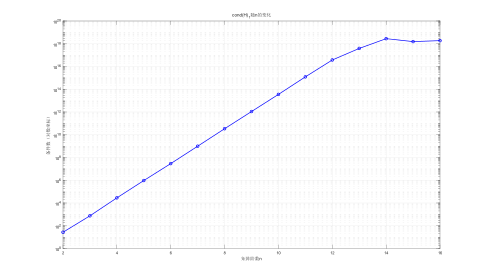
\includegraphics{1.pdf} 
    \caption{Hilbert 矩阵条件数随阶数 $n$ 的变化 (半对数坐标)}
    \label{fig:cond}
\end{figure}
在单对数坐标系下,条件数曲线呈现明显的线性增长趋势,说明Hilbert矩阵的条件数随阶数$n$呈指数级增长。

当$n=13$左右时,条件数达到了$10^{18}$量级。此时矩阵的数值性质已极度不稳定,计算出的条件数出现波动,不再严格单调。

\subsubsection{n=6 时的求解误差对比}
当$n=6$时,各方法的求解结果及误差如下表所示:

\begin{table}[h]
    \centering
    \caption{不同方法求解 $H_6 x = b_6$ 的误差对比($n=6$)}
    \begin{tabular}{lccl}
        \hline
        \textbf{方法} & \textbf{迭代次数} & \textbf{相对误差} & \textbf{状态分析} \\
        \hline
        LU 分解 & - & $2.2057 \times 10^{-10}$ & 有效,但精度受限 \\
        Jacobi & 5000 & NaN & 发散\\
        SOR ($\omega=1.0$) & 5000 & $2.5376 \times 10^{-2}$ & 收敛停滞 \\
        SOR ($\omega=1.25$) & 5000 & $2.8683 \times 10^{-2}$ & 效果变差 \\
        SOR ($\omega=1.5$) & 5000 & $3.2851 \times 10^{-2}$ & 效果更差 \\
        CG (共轭梯度) & 5 & $5.4680 \times 10^{-3}$ & 假性收敛 \\
        \hline
    \end{tabular}
    \label{tab:n6_error}
\end{table}

Jacobi发散,结果出现NaN,Hilbert矩阵不满足Jacobi方法收敛所需的严格对角占优条件,导致迭代过程中数值溢出。

LU分解精度最高,在$n=6$时,矩阵$\mathrm{cond} \approx 10^7$较大,LU分解仍能保持约10位有效数字的精度。

迭代法效果有限,SOR和共轭梯度法最终误差停留在$10^{-2}$到$10^{-3}$。

\subsubsection{误差随阶数 n 的变化}
随着$n$增大,各方法相对误差的变化曲线如图 \ref{fig:error_trend} 所示。

\begin{figure}[h]
    \centering
    % 【修改】直接引用生成的 PDF 文件
    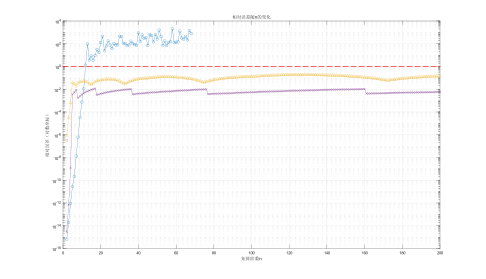
\includegraphics{2.pdf} 
    \caption{各方法相对误差随矩阵阶数 $n$ 的变化趋势}
    \label{fig:error_trend}
\end{figure}
LU分解(蓝色)在$n < 10$时,误差随$n$迅速上升,从$10^{-15}$上升至$10^{-2}$)。当$n=12$时,相对误差超过100\%,计算结果已完全失去有效数字,数值求解失效。

迭代法(黄色和紫色)曲线始终位于$10^{-2}$左右,精度停滞,难以继续提升。

\section{总结}
    1. 通过 Hilbert 矩阵实验,深刻理解了条件数 $\mathrm{cond}(A)$ 对数值稳定性的决定性作用。当 $\mathrm{cond}(A)$ 很大时,微小的扰动(如计算机舍入误差)会被显著放大。

    2. 对于病态方程组,直接法(如LU)比简单的迭代法更可靠,但需要使用高精度计算。

\end{document}